\chapter{Question1}
\section{问题概述}
%
%%对问题的直观描述
%
本问题要求实现二元感知器。

%
%对项目已有代码的阅读和理解
%

%
%解决问题的思路和想法
%

\section{算法设计}
%
%用自己的语言描述解决问题所使用的算法的原理及功能,设计思路和算法流程图
%
这里假设所给的数据是可以被线性函数所完全分隔分隔开来的。对于二分类问题,感知器通过自身权重向量于数据的特征向量之间的点积的符号来进行分类。
对于正例,点积符号为正,感知器输出1;对于负例,点积符号为负,感知器输出-1。为了使得感知器能够将数据的正负例完全分离开来,需要进行学习,即根据分类结果
不断对感知器中的权重进行调整。

如果感知器给出的分类结果与真实类别一致,则无需进行调整。否则,说明点积
\[\mathbf{W}\cdot\mathbf{x}\]
的符号错误,其中$\mathbf{W}$为感知器的权重向量,$\mathbf{x}$为样例的特征向量。为此,如果感知器返回的点积为正,需要调整权重向量使其返回的点积
减小;如果感知器返回的点积为负,需要调整权重向量使其返回的点积增大。由于$\mathbf{x}\cdot\mathbf{x}\geq 0$,所以可以将$\mathbf{W}$
调整为
\[\mathbf{W}^{\prime}=\mathbf{W}-\mathbf{sgn}(\mathbf{W}\cdot\mathbf{x})\mathbf{x},\]
从而有
\[\mathbf{W}^{\prime}\cdot\mathbf{x}=\mathbf{W}\cdot\mathbf{x}-\mathbf{sgn}(\mathbf{W}\cdot\mathbf{x})\mathbf{x}\cdot\mathbf{x},\]
达到了上述的需求。

只需不断调整,直到感知器能够完全正确分类所有样例即可。
\section{算法实现}
%
%在算法原理的基础上,结合代码,讲述算法的实现细节、核心函数、模块输入输出,数据结构定义等内容
%
%
\begin{lstlisting}[emph={[3]dataset,x},emphstyle={[3]\color{vscode_parametercolor}},emph={[4]GameState,MinimaxAgent,AlphaBetaAgent},emphstyle={[4]\color{vscode_classcolor}}]
def run(self, x):
    return nn.DotProduct(x,self.w)

def get_prediction(self, x):
    return 1 if nn.as_scalar(self.run(x)) >= 0 else -1

def train(self, dataset):
    while True:
        OK = True
        for x,y in dataset.iterate_once(1):
            res = self.get_prediction(x)
            if nn.as_scalar(y) != res:
                self.w.update(x,-res)
                OK = False
                break
        if OK:
            break
\end{lstlisting}

\section{实验结果}
我成功获得了本问题的所有分数。本问所用的测试样例便是一个二元分类问题,要求感知器能够正确分类所有样例。
\begin{figure}[htbp]
    \centering
    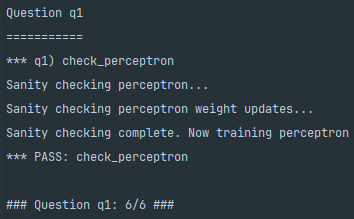
\includegraphics{pic/q1.png}
    \caption{Question1实验结果}\label{q1}
\end{figure}
%
%实验中遇到的问题及解决方案,收获和思考:对算法的理解、优缺点的评价、算法的适用场景
%
